%%
%% This is file `sample-sigconf.tex',
%% generated with the docstrip utility.
%%
%% The original source files were:
%%
%% samples.dtx  (with options: `all,proceedings,bibtex,sigconf')
%% 
%% IMPORTANT NOTICE:
%% 
%% For the copyright see the source file.
%% 
%% Any modified versions of this file must be renamed
%% with new filenames distinct from sample-sigconf.tex.
%% 
%% For distribution of the original source see the terms
%% for copying and modification in the file samples.dtx.
%% 
%% This generated file may be distributed as long as the
%% original source files, as listed above, are part of the
%% same distribution. (The sources need not necessarily be
%% in the same archive or directory.)
%%
%%
%% Commands for TeXCount
%TC:macro \cite [option:text,text]
%TC:macro \citep [option:text,text]
%TC:macro \citet [option:text,text]
%TC:envir table 0 1
%TC:envir table* 0 1
%TC:envir tabular [ignore] word
%TC:envir displaymath 0 word
%TC:envir math 0 word
%TC:envir comment 0 0
%%
%% The first command in your LaTeX source must be the \documentclass
%% command.
%%
%% For submission and review of your manuscript please change the
%% command to \documentclass[manuscript, screen, review]{acmart}.
%%
%% When submitting camera ready or to TAPS, please change the command
%% to \documentclass[sigconf]{acmart} or whichever template is required
%% for your publication.
%%
%%
\documentclass[sigconf, authorversion, nonacm, screen]{acmart}
%%
%% \BibTeX command to typeset BibTeX logo in the docs
\AtBeginDocument{%
  \providecommand\BibTeX{{%
    Bib\TeX}}}

%% Rights management information.  This information is sent to you
%% when you complete the rights form.  These commands have SAMPLE
%% values in them; it is your responsibility as an author to replace
%% the commands and values with those provided to you when you
%% complete the rights form.

%\setcopyright{acmlicensed}
%\copyrightyear{2025}
%\acmYear{2018}
%\acmDOI{XXXXXXX.XXXXXXX}

%% These commands are for a PROCEEDINGS abstract or paper.

%\acmConference[Conference acronym 'XX]{Make sure to enter the correct
%  conference title from your rights confirmation email}{June 03--05,
%  2018}{Woodstock, NY}

%%
%%  Uncomment \acmBooktitle if the title of the proceedings is different
%%  from ``Proceedings of ...''!
%%
%%\acmBooktitle{Woodstock '18: ACM Symposium on Neural Gaze Detection,
%%  June 03--05, 2018, Woodstock, NY}

%\acmISBN{978-1-4503-XXXX-X/2018/06}


%%
%% Submission ID.
%% Use this when submitting an article to a sponsored event. You'll
%% receive a unique submission ID from the organizers
%% of the event, and this ID should be used as the parameter to this command.
%%\acmSubmissionID{123-A56-BU3}

%%
%% For managing citations, it is recommended to use bibliography
%% files in BibTeX format.
%%
%% You can then either use BibTeX with the ACM-Reference-Format style,
%% or BibLaTeX with the acmnumeric or acmauthoryear sytles, that include
%% support for advanced citation of software artefact from the
%% biblatex-software package, also separately available on CTAN.
%%
%% Look at the sample-*-biblatex.tex files for templates showcasing
%% the biblatex styles.
%%

%%
%% The majority of ACM publications use numbered citations and
%% references.  The command \citestyle{authoryear} switches to the
%% "author year" style.
%%
%% If you are preparing content for an event
%% sponsored by ACM SIGGRAPH, you must use the "author year" style of
%% citations and references.
%% Uncommenting
%% the next command will enable that style.
%%\citestyle{acmauthoryear}


%%
%% end of the preamble, start of the body of the document source.
\begin{document}

%%
%% The "title" command has an optional parameter,
%% allowing the author to define a "short title" to be used in page headers.
\title{Broken Morals}

%%
%% The "author" command and its associated commands are used to define
%% the authors and their affiliations.
%% Of note is the shared affiliation of the first two authors, and the
%% "authornote" and "authornotemark" commands
%% used to denote shared contribution to the research.
\author{Emanuele Messina}
\author{Nicola Bavaro}
\author{Rolf Erik Appel}
\author{Mozhdeh Hajiani}
%\authornote{Both authors contributed equally to this research.}
\email{giuseppeemanuele.messina@studenti.polito.it}
\email{nicola.bavaro@studenti.polito.it}
\email{rolferik.appel@studenti.polito.it}
\email{mozhdeh.hajiani@studenti.polito.it}
%\orcid{1234-5678-9012}
%\authornotemark[1]
%\email{webmaster@marysville-ohio.com}
\affiliation{%
  \institution{Politecnico di Torino}
  \city{Torino}
  \country{Italy}
}

\begin{comment}
\author{Lars Th{\o}rv{\"a}ld}
\affiliation{%
  \institution{The Th{\o}rv{\"a}ld Group}
  \city{Hekla}
  \country{Iceland}}
\email{larst@affiliation.org}
\end{comment}

%%
%% By default, the full list of authors will be used in the page
%% headers. Often, this list is too long, and will overlap
%% other information printed in the page headers. This command allows
%% the author to define a more concise list
%% of authors' names for this purpose.
\renewcommand{\shortauthors}{E. Messina, N. Bavaro, R. E. Appel and M. Hajiani}

%%
%% The abstract is a short summary of the work to be presented in the
%% article.
\begin{abstract}
Organizational moral misalignment is very important because ethical blind spots can lead to reputational damage, internal conflict, and poor decision-making.
In tackling organizational moral misalignment, related work often failed to incorporate diverse perspectives within the company before decisions are made, instead relying on static top-down ethics reviews or individual assessments. 
To partly tackle this limitation, we make three contributions. 
First, we develop a software tool that uses AI agents to simulate the perspectives of a CEO, an ethicist, and an engineer. Given a moral dilemma, the tool generates a summary of the agents' responses and presents it to the user to support their decision-making.
Second, we evaluate the effectiveness of our tool through a controlled study with 50 senior technology professionals, from director level to CEO. Each participant is shown one of five business ethics dilemmas that collectively cover all the foundations declared in moral foundation theory, and tasked with providing their justification. Half of the participants are also shown the tool's summary for the given dilemma. All justifications are evaluated using a six-dimensional scoring rubric designed to assess the quality and sophistication of ethical reasoning.
Third, we show that exposure to our tool leads to more nuanced ethical justifications [...].

 TODO CHECK PAPER WRITING CHECKLIST
\end{abstract}

%%
%% The code below is generated by the tool at http://dl.acm.org/ccs.cfm.
%% Please copy and paste the code instead of the example below.
%%
\begin{CCSXML}
<ccs2012>
   <concept>
       <concept_id>10010405.10010455.10010461</concept_id>
       <concept_desc>Applied computing~Sociology</concept_desc>
       <concept_significance>500</concept_significance>
       </concept>
   <concept>
       <concept_id>10010147.10010178.10010219.10010220</concept_id>
       <concept_desc>Computing methodologies~Multi-agent systems</concept_desc>
       <concept_significance>300</concept_significance>
       </concept>
 </ccs2012>
\end{CCSXML}

\ccsdesc[500]{Applied computing~Sociology}
\ccsdesc[300]{Computing methodologies~Multi-agent systems}

%%
%% Keywords. The author(s) should pick words that accurately describe
%% the work being presented. Separate the keywords with commas.
\keywords{business ethics, organizational decision-making, large language models, moral misalignment, AI deliberation, Plurals framework, ethical reasoning, prototype evaluation, decision support systems}

%% A "teaser" image appears between the author and affiliation
%% information and the body of the document, and typically spans the
%% page.
\begin{teaserfigure}
  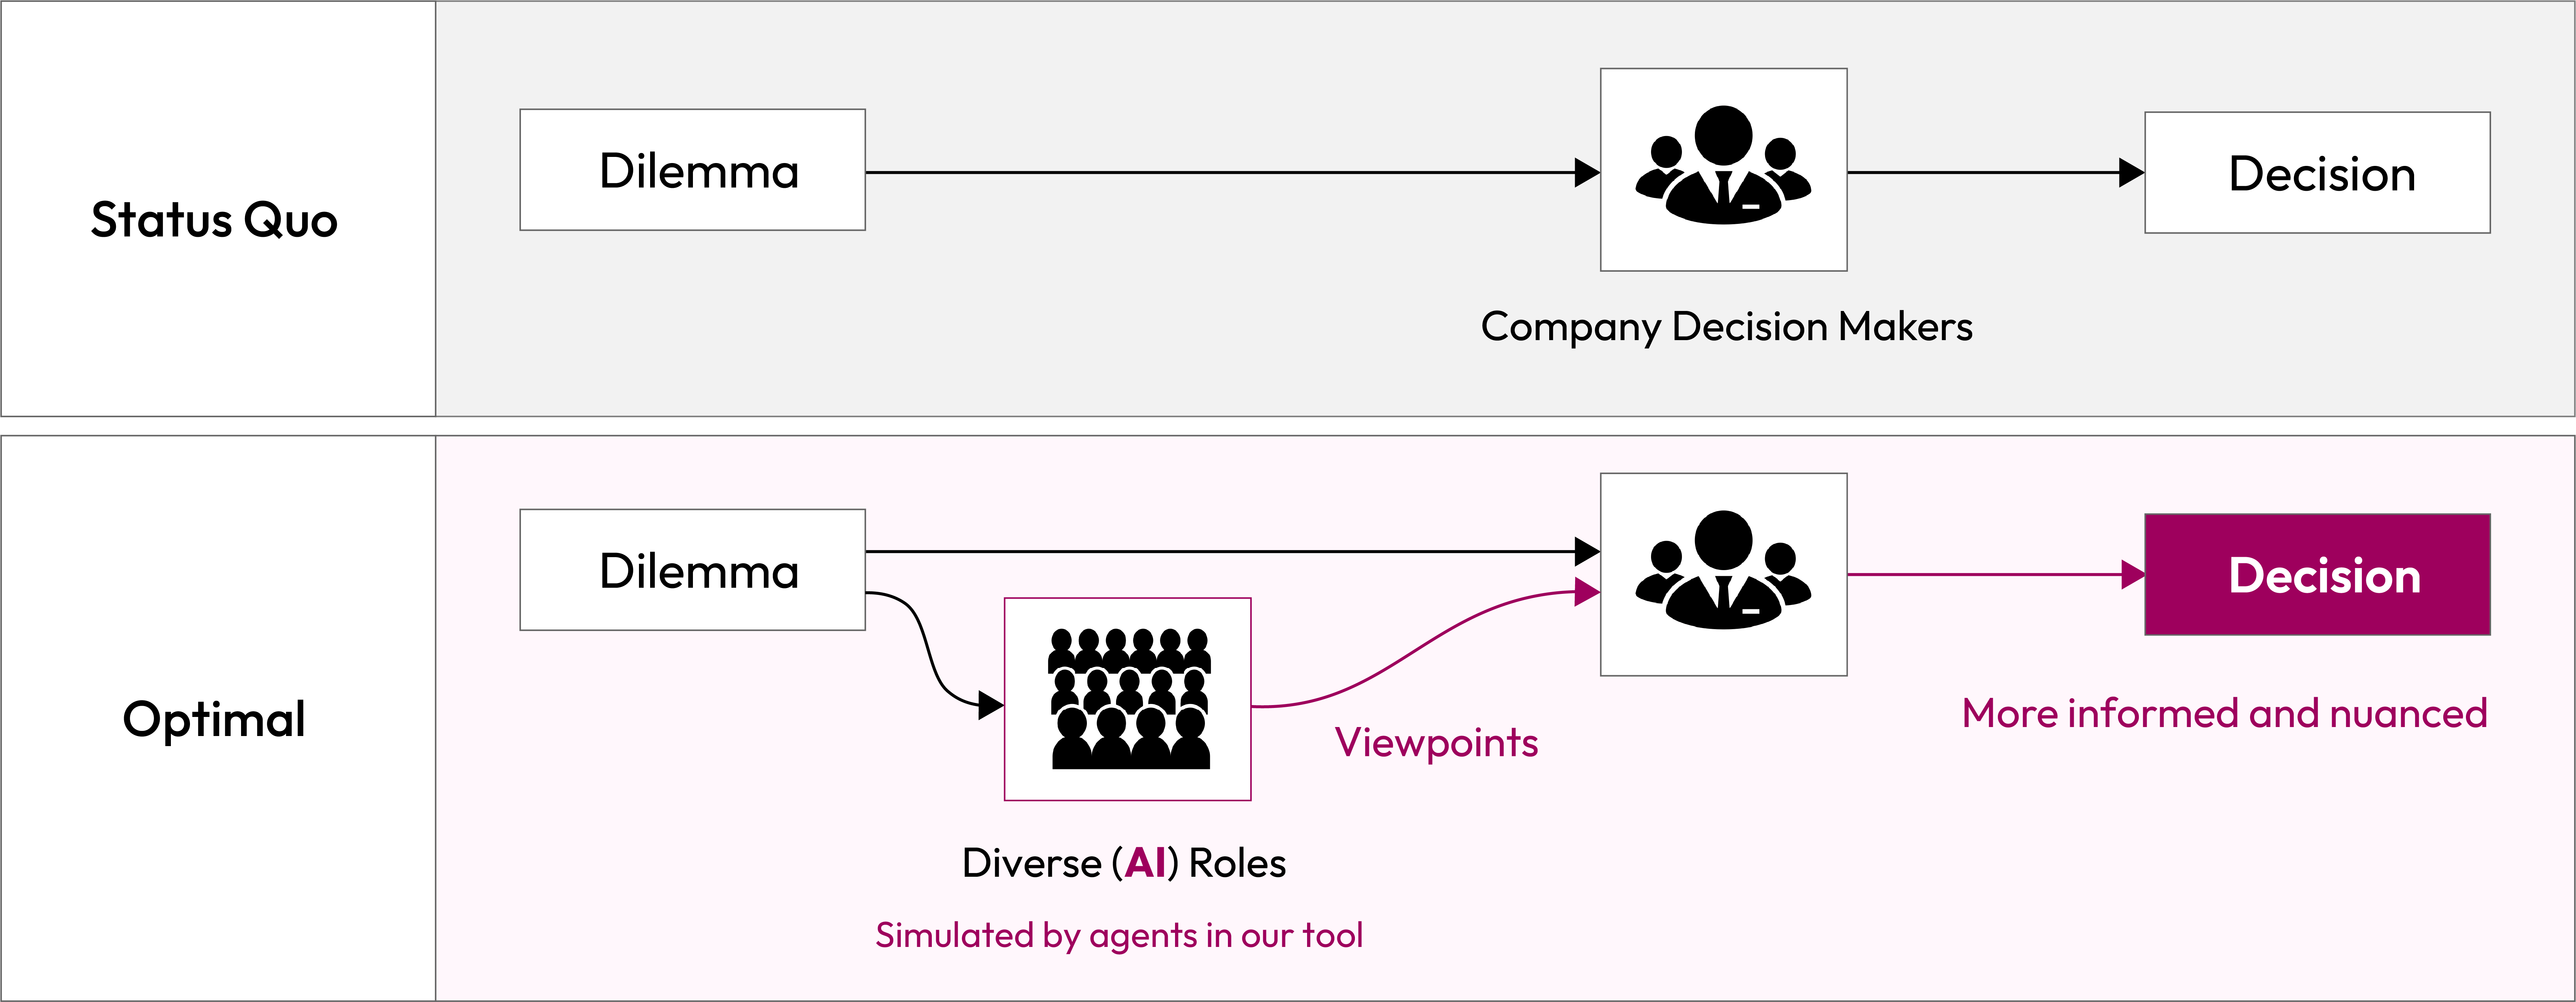
\includegraphics[width=\textwidth]{teaser}
  \caption{Overview of the Broken Morals project. (\textit{Status Quo}) Usually, company decisions are taken without including the perspectives of different roles. (\textit{Optimal}) We show that the exposure to those perspectives and viewpoints leads decision-makers to take decisions that are more relevant, useful and aware of contextual conditions.}
  \Description{Overview of the Broken Morals project}
  \label{fig:teaser}
\end{teaserfigure}

\received{2 June 2025}
\begin{comment}
\received[revised]{12 March 2009}
\received[accepted]{5 June 2009}
\end{comment}

%%
%% This command processes the author and affiliation and title
%% information and builds the first part of the formatted document.
\maketitle

\section{Related Work}

%TODO RELATED WORK

%Don’t review everything under the sun. Focus only on Problem Y.
%• Keep it to one page. If it drags on, you’re overcompensating.
%• End with this line: "To sum up, previous work has failed to address Y." Boom.
%• Can’t pinpoint a clear Y? Rewrite your Abstract/Intro/Related Work

\section{Methods}

TODO METHODS

\begin{comment}
Here you explain how you’ve solved the problem 
in our case 

SITUATION: Problem X is very important because . . .
COMPLICATION: In tackling problem X, related work failed in doing Y
PROPOSAL: To partly tackle Y, we make N contributions [list of contributions]

X = organizational moral misalignment
Y = incorporating different perspectives

we solve the problem of incorporating different perspectives
so we explain how we did it
\end{comment}

\subsection{Proposal}

To incorporate perspectives of different organizational roles when making company decisions,
we propose a novel software tool.
The tool is intended to be used by company decision makers when taking decisions on internal dilemmas,
with the goal of making more informed decisions.
The user inputs a moral dilemma in the tool, and the tool gives the user a summary as output.
Internally, the tool simulates a deliberation among AI agents representing different organizational roles, on the given dilemma.
A moderator agent poses the dilemma to the other agents, oversees the discussion and finally generates the summary drawing from the deliberation transcript.
The moderator generates the final summary by extracting the key points in which the role-based agents agreed and disagreed during the discussion, 
and a list of key points and/or questions that the end user should cover when answering the dilemma.
The summary thus contains three paragraphs: areas of agreement, areas of disagreement and practical points for the user to cover when answering the dilemma.
The purpose of this summary is to make the user think critically about the dilemma
without forcing or inducing a particular point of view, 
but rather aiding their thought process and enriching their final response 
with aspects they might not consider due to lack of efficient communication with other work figures,
as well as other psychological reasons such as underestimating or misunderstanding the dilemma itself and its implications.
The proposed behavior for this tool is general and can be implemented in various ways: varying the number of agents and their roles, the topology in which they discuss, and the type of moderation they are subjected to.
The following section describes specifically the implementation we developed and tested in the context of this study.

\subsection{Implementation}

For this pilot study we decided to implement a simple prototype of the proposed tool for the purpose of testing.
We implemented the AI agents and their deliberation using the Plurals [TODO CITE] framework: a Python library that orchestrates AI agents to allow pluralistic AI deliberations.
Plurals eases the definition of agents, discussion topologies and moderators, and provides an abstraction layer over several LLM API backends.
We used GPT-4.1 as the underlying LLM for each agent and the moderator.
We defined three AI agent personas to represent three specific roles inside a generic technology company: a Chief Executive Officer (CEO), an Ethicist and a generic Engineer [APPENDIX LINK].
We used the default moderator persona offered by Plurals: an expert impartial moderator overseeing a given task.
In Plurals, both the agents and the moderator are aware of a common task which is generally the goal that should be achieved by the simulation.
In our case, the task is to provide and answer to the given dilemma, expressing thoughts and opinions [APPENDIX LINK].

Refer to the [APPENDIX] to see the exact prompts we used.

-the moderator poses the dilemma
-the topology is ensemble, everyone is at the same level, they respond independently to get each viewpoint without undermining anyone based on their hierarchy level
for this study we chose 3 roles ceo ethicist engineer
-the moderator generates a summary with agreement disagreement points between the agents justifications and a list of practical points/questions for the user to cover when answering the original dilemma
this way the user is not biased towards an artificial opinion but instead is pushed towards considering the different perspectives thus to take more informed decisions.

see appendix for the specific prompts

\section{Evaluation}

TODO EVALUATION

The goal of our tool is to help company decision-makers make better decisions with respect to the status quo.
To ascertain the effectiveness of our tool at meeting this goal, we conducted a user study with people in tech to verify that the answers in the treatment group scored better than control with respect to a rubric we created, for a set of dilemmas we selected.
Additionally, we wanted to see if, overall, there was a time difference in the responding between the two groups, and if participants in the treatment group appreciated the tool summary as an aid when answering.

To measure our metrics, we 
1) selected the dilemmas
2) recruited people
3) divided into control and treatment, with minutes and pay and task
4) created a rubric 
5) scored the answers

\subsection{Dilemma Selection}
scu dataset, mfc classifier
\subsection{Participants Recruitment}
prolific, roles
\subsection{Participant Groups and Tasks}
control, treatment, form format, pay, time, task, questionnaires
\subsection{Evaluation Rubric}
To compare the quality of answers across the Control and Treatment groups, we needed a way to evaluate responses in a consistent and meaningful way. Since moral dilemmas invite complex, subjective reasoning, we could not rely on simple or automatic measures. Instead, we designed an evaluation rubric that breaks down each response into clear dimensions, allowing us to assess specific aspects of reasoning and communication.

We began by reviewing previous research in areas such as argumentation, dialogue systems, ethical reasoning, and decision-making. Based on this review, we identified six dimensions that best reflect the qualities we wanted to measure. Each dimension is supported by existing literature and was selected to match the goals of our study.

\begin{itemize}
  \item \textit{Clarity and Structure.} Does the response express its ideas clearly? Is the reasoning easy to follow and well-organized?\\
  \hspace*{0.5em}Based on McTear (2005), who highlights the importance of structure and readability in effective communication.

  \item \textit{Relevance.} Does the response stay focused on the moral dilemma? Are the points made directly connected to the question?\\
  \hspace*{0.5em}Informed by Habernal and Gurevych (2016), who show that content relevance strengthens argument quality.

  \item \textit{Persuasiveness.} Is the argument convincing? Does it use logic, appropriate tone, and structure to support its claims?\\
  \hspace*{0.5em}Draws from Johnson and Blair (2006), who emphasize the role of logical and well-structured reasoning in persuasion.

  \item \textit{Concern for Long-Term Consequences.} Does the response consider future or societal effects of the proposed action?\\
  \hspace*{0.5em}Inspired by the Impact Assessment Card (CSCW~'25), which promotes ethical foresight.

  \item \textit{Practical Usefulness.} Is the proposed solution realistic? Could it work in practice?\\
  \hspace*{0.5em}Based on Bazerman and Moore (2012), who stress the importance of actionable and realistic decision-making.

  \item \textit{Awareness of Context.} Does the response take into account the social, cultural, or situational context of the dilemma?\\
  \hspace*{0.5em}Also from the Impact Assessment Card (CSCW~'25), which encourages attention to contextual factors in ethical reasoning.
\end{itemize}

Each dimension was defined using a 5-point Likert scale, ranging from 1 (``very low'') to 5 (``very high''). The rubric itself provided the conceptual framework for evaluating responses, while the actual scoring procedure is described in the following section.


\subsection{Scoring the Answers}
Evaluating subjective responses is inherently challenging, especially when the goal is to compare two groups fairly. To ensure our ratings were both unbiased and reliable, we followed a structured scoring process based on the evaluation rubric described above.

We began by generating three identical scoring files---one for each rater. Each file contained an \texttt{AnswerID} and the six rubric dimensions, but no information about whether the response came from the Control or Treatment group. This ensured that all evaluations were blind to condition.

Each rater independently assigned scores using the 5-point Likert scale across all dimensions. Once all ratings were completed, we reattached the group labels to the responses and calculated inter-rater reliability using Fleiss' Kappa for each dimension. We computed agreement scores separately for Control, Treatment, and the full dataset. Our target was to achieve a Kappa score above 0.6 for all dimensions---commonly accepted as the threshold for substantial agreement.

Initial scores fell short of this threshold in some cases. To address this, we held a calibration session where raters discussed discrepancies, reviewed selected responses, and refined their understanding of the rubric. After this reconciliation, we repeated the scoring where needed and achieved the following agreement levels:

\begin{table}[H]
\centering
\caption{Fleiss' Kappa Scores by Dimension and Group}
\begin{tabular}{lccc}
\toprule
\textbf{Dimension} & \textbf{Control} & \textbf{Treatment} & \textbf{Total} \\
\midrule
Clarity & 0.669 & 0.617 & 0.645 \\
Relevance & 0.746 & 0.701 & 0.733 \\
Persuasiveness & 0.756 & 0.600 & 0.681 \\
Concern for Long-Term Consequences & 0.735 & 0.599 & 0.671 \\
Practical Usefulness & 0.754 & 0.606 & 0.683 \\
Awareness of Context & 0.715 & 0.612 & 0.667 \\
\bottomrule
\end{tabular}
\label{tab:kappa}
\end{table}


With these agreement levels in place, we computed the average score across raters for each dimension. This resulted in a final dataset with the following structure: \texttt{AnswerID}, \texttt{DilemmaID}, \texttt{Group}, followed by the six rubric scores. This dataset served as the foundation for the subsequent statistical analysis.



\subsection{Results}

discuss rater agreement differences if present
discuss statistical tests and what they show, both rubric and questionnaires

\section{Discussion}
TODO DISCUSSION

Here you discuss how your results are: (1) in-line with previous work; and (2) differ
(expand) on previous work. Also, you can list the limitations of your work (link to future work)

(a) Which results match previous findings in the literature?
(b) Which results differ from previous findings, and why

\section{Future Work}

Study with more participants
Participants from different roles, countries, industries
Use more dilemmas from dataset
Test more Plurals configurations
Different topologies
Different/more roles
Compare with single vanilla LLM
Study to codesign the tool
Understand which exact requirements a tools like ours should have to support real world decisions


\section{Tables}

The ``\verb|acmart|'' document class includes the ``\verb|booktabs|''
package --- \url{https://ctan.org/pkg/booktabs} --- for preparing
high-quality tables.

Table captions are placed {\itshape above} the table.

Because tables cannot be split across pages, the best placement for
them is typically the top of the page nearest their initial cite.  To
ensure this proper ``floating'' placement of tables, use the
environment \textbf{table} to enclose the table's contents and the
table caption.  The contents of the table itself must go in the
\textbf{tabular} environment, to be aligned properly in rows and
columns, with the desired horizontal and vertical rules.  Again,
detailed instructions on \textbf{tabular} material are found in the
\textit{\LaTeX\ User's Guide}.

Immediately following this sentence is the point at which
Table~\ref{tab:freq} is included in the input file; compare the
placement of the table here with the table in the printed output of
this document.

\begin{table}
  \caption{Frequency of Special Characters}
  \label{tab:freq}
  \begin{tabular}{ccl}
    \toprule
    Non-English or Math&Frequency&Comments\\
    \midrule
    \O & 1 in 1,000& For Swedish names\\
    $\pi$ & 1 in 5& Common in math\\
    \$ & 4 in 5 & Used in business\\
    $\Psi^2_1$ & 1 in 40,000& Unexplained usage\\
  \bottomrule
\end{tabular}
\end{table}

To set a wider table, which takes up the whole width of the page's
live area, use the environment \textbf{table*} to enclose the table's
contents and the table caption.  As with a single-column table, this
wide table will ``float'' to a location deemed more
desirable. Immediately following this sentence is the point at which
Table~\ref{tab:commands} is included in the input file; again, it is
instructive to compare the placement of the table here with the table
in the printed output of this document.

\begin{table*}
  \caption{Some Typical Commands}
  \label{tab:commands}
  \begin{tabular}{ccl}
    \toprule
    Command &A Number & Comments\\
    \midrule
    \texttt{{\char'134}author} & 100& Author \\
    \texttt{{\char'134}table}& 300 & For tables\\
    \texttt{{\char'134}table*}& 400& For wider tables\\
    \bottomrule
  \end{tabular}
\end{table*}

Always use midrule to separate table header rows from data rows, and
use it only for this purpose. This enables assistive technologies to
recognise table headers and support their users in navigating tables
more easily.

\section{Math Equations}


\subsection{Inline (In-text) Equations}
A formula that appears in the running text is called an inline or
in-text formula.  It is produced by the \textbf{math} environment,
which can be invoked with the usual
\texttt{{\char'134}begin\,\ldots{\char'134}end} construction or with
the short form \texttt{\$\,\ldots\$}. You can use any of the symbols
and structures, from $\alpha$ to $\omega$, available in
\LaTeX~\cite{Lamport:LaTeX}; this section will simply show a few
examples of in-text equations in context. Notice how this equation:
\begin{math}
  \lim_{n\rightarrow \infty}x=0
\end{math},
set here in in-line math style, looks slightly different when
set in display style.  (See next section).

\subsection{Display Equations}
A numbered display equation---one set off by vertical space from the
text and centered horizontally---is produced by the \textbf{equation}
environment. An unnumbered display equation is produced by the
\textbf{displaymath} environment.

Again, in either environment, you can use any of the symbols and
structures available in \LaTeX\@; this section will just give a couple
of examples of display equations in context.  First, consider the
equation, shown as an inline equation above:
\begin{equation}
  \lim_{n\rightarrow \infty}x=0
\end{equation}
Notice how it is formatted somewhat differently in
the \textbf{displaymath}
environment.  Now, we'll enter an unnumbered equation:
\begin{displaymath}
  \sum_{i=0}^{\infty} x + 1
\end{displaymath}
and follow it with another numbered equation:
\begin{equation}
  \sum_{i=0}^{\infty}x_i=\int_{0}^{\pi+2} f
\end{equation}
just to demonstrate \LaTeX's able handling of numbering.

\section{Figures}

The ``\verb|figure|'' environment should be used for figures. One or
more images can be placed within a figure. If your figure contains
third-party material, you must clearly identify it as such, as shown
in the example below.
\begin{figure}[h]
  \centering
  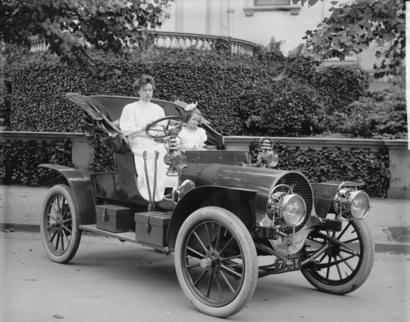
\includegraphics[width=\linewidth]{sample-franklin}
  \caption{1907 Franklin Model D roadster. Photograph by Harris \&
    Ewing, Inc. [Public domain], via Wikimedia
    Commons. (\url{https://goo.gl/VLCRBB}).}
  \Description{A woman and a girl in white dresses sit in an open car.}
\end{figure}

Your figures should contain a caption which describes the figure to
the reader.

Figure captions are placed {\itshape below} the figure.

Every figure should also have a figure description unless it is purely
decorative. These descriptions convey what’s in the image to someone
who cannot see it. They are also used by search engine crawlers for
indexing images, and when images cannot be loaded.

A figure description must be unformatted plain text less than 2000
characters long (including spaces).  {\bfseries Figure descriptions
  should not repeat the figure caption – their purpose is to capture
  important information that is not already provided in the caption or
  the main text of the paper.} For figures that convey important and
complex new information, a short text description may not be
adequate. More complex alternative descriptions can be placed in an
appendix and referenced in a short figure description. For example,
provide a data table capturing the information in a bar chart, or a
structured list representing a graph.  For additional information
regarding how best to write figure descriptions and why doing this is
so important, please see
\url{https://www.acm.org/publications/taps/describing-figures/}.

%%
%% The acknowledgments section is defined using the "acks" environment
%% (and NOT an unnumbered section). This ensures the proper
%% identification of the section in the article metadata, and the
%% consistent spelling of the heading.
\begin{acks}
The authors thank Prof. Daniele Quercia and Dr. Edyta Bogucka for their valuable guidance and support of this research. We also acknowledge Nokia Bell Labs for providing the funding that made this research possible.
\end{acks}

%%
%% The next two lines define the bibliography style to be used, and
%% the bibliography file.
\bibliographystyle{ACM-Reference-Format}
\bibliography{sample-base}


%%
%% If your work has an appendix, this is the place to put it.
\appendix

\section{Ethical considerations}

This study was conducted in accordance with general ethical guidelines for research with human participants, ensuring respect for participant autonomy, privacy, and well-being.
Participants were recruited voluntarily through Prolific, a reputable online platform for academic studies, using its standard informed consent procedures and screening tools to select senior technology professionals ranging from director level to chief executive officers. No coercion or undue influence was involved in recruitment.
The study exposed participants to automatically generated summaries created by artificial intelligence agents simulating organizational roles. These agents do not represent real individuals; their responses were generated based on predefined prompts and models. Participants were informed that these simulated perspectives were intended to assist their ethical decision-making and should not be considered definitive answers.
All ethical dilemmas presented were non-sensitive business ethics scenarios drawn from publicly available sources. 
No personally identifiable or health-related information was collected beyond Prolific’s internal IDs, which were removed before publishing the anonymized study data to further protect participant anonymity.
Participants were free to withdraw from the study at any time without penalty. The materials and procedures posed no known risks or distress.

\section{Authors' Positionality Statement}

We are master’s students at Politecnico di Torino from diverse backgrounds and nationalities.
Out teams is comprised of two Italians, one Iranian, and one Danish. 
Our specializations are Data Science, Computer Engineering, Artificial Intelligence and Design and Innovation.
Our team’s strength lies in its global and interdisciplinary makeup. This diversity in ethnic and interdisciplinary expertise let us leverage varied approaches and viewpoints to ensure a thorough and well-rounded study. 
We are aware that our backgrounds influence how we conducted the research and interpreted the data. 
We acknowledge that our perspectives might shape the way we framed ethical dilemmas and analyzed responses.
We have critically reflected on these potential biases throughout the project to promote transparency and ethical rigor. 
We encourage readers to consider how our positionality may affect the findings.

\section{Division of Labour}

While certain areas of the project had clear leads to leverage each team member’s expertise, many tasks were collaboratively shared across the team.

\textbf{Major Contributions:}
\begin{itemize}
  \item {Emanuele Messina:} Developed the Plurals software code and prompts, conducted the Prolific study, created graphics, and coordinated overall project management.
  \item {Rolf Erik Appel:} Led the presentation pitch and business study, and compiled the RAI cards.
  \item {Nicola Bavaro:} Developed code for dilemma selection and data analysis, led data analysis and interpretation, and developed the evaluation rubric with supporting references.
  \item {Mozhdeh Hajiani:} Performed dilemma selection coding, developed the evaluation rubric with supporting references, led related work research, and provided analysis support.
\end{itemize}

\textbf{Shared Efforts:}
\begin{itemize}
  \item All members participated in reviewing and refining the evaluation rubric.
  \item All members collaborated in refining dilemma selection to ensure clarity, feasibility, diversity, and validation of automatic classification.
  \item The team jointly contributed to writing and revising the manuscript, ensuring a cohesive and polished final paper.
\end{itemize}

The diverse ideas and viewpoints of all team members were essential and carefully considered throughout the project, making its successful completion possible.

\section{More stuff}

TODO

\subsection{That we didn't put}

In the 8 pages, like the tables with the exact numbers of answers and evaluations.

\section{Online Resources}

TODO
github repo, video pitch, business feasibility study, rai guidelines


\end{document}
\endinput
%%
%% End of file `sample-sigconf.tex'.
